\chapter{Direct methods for solving linear systems \todol{todo}}

%\noindent
%\todop{
%\begin{itemize}
%    \item Dense ldl (left looking) 
%    \item Sparse (+ supernodes) 
%    \item Permutation fill in
%    \item Parallelization (ND) 
%    \item Solve 
%    \item
%    \item Elimination tree? 
%    \item
%    \item
%    \item Different types of factorization (LU, Cholesky, LDL')
%    \item Solving system (Equation)
%    \item Permutation (fill-in reducing)
%    \item Supernodes (performance)
%\end{itemize}
%}
%
Let $A$ be an $N \times N$ symmetric indefinite matrix and $x$ and $b$ be vectors of size $N$.
The linear system $A x = b$ is solved via $LDL^T$ decomposition by factorizing $A$ into an unit lower diagonal matrix $L$ and a diagonal matrix $D$ so that $A = LDL^T$.
The system is then solved in three steps. First, $Ly=b$ is solved via forward substitution. This is followed by a diagonal solve $Dz=y$ and afterwards the resulting $z$ vector is used to solve for the solution vector  $L^Tx=z$ via backward substitution.

%
%
%\section{Matrix permutation (fill-in reduction, parallelization)}
%
%\section{Sparse triangular solve}
%
\section{$LDL^T$ factorization}

The Left-looking $LDL^T$ factorization algorithm can be derived from the equation \ref{eq:ldl}.

\begin{equation}
    \begin{bmatrix}
        A_{11} & A_{21}^T & A_{31}^T \\
        A_{21} & a_{22} & A_{32}^T \\
        A_{31} & A_{32} & A_{33} \\
    \end{bmatrix}
    =
    \begin{bmatrix}
        L_{11} & & \\
        L_{21} & 1 & \\
        L_{31} & L_{32} & L_{33} \\
    \end{bmatrix}
    *
    \begin{bmatrix}
        D_{11} & & \\
        & d_{22} & \\
        & & D_{33} \\
    \end{bmatrix}
    *
    \begin{bmatrix}
        L_{11}^T & L_{21}^T & L_{31}^T \\
        & 1 & L_{32}^T \\
        & & L_{33}^T \\
    \end{bmatrix}
    \label{eq:ldl}
\end{equation}

The factors L and D are computed one column at a time from left to right. In equation~\ref{eq:ldl} the matrices are decomposed into blocks. The first column corresponds to columns 1 to k-1 that are already computed, the second column represents column $k$ being computed and the third column (columns k+1 to n) will be computed later.

With this decomposition, we can form two equations:

\begin{eqnarray}
    L_{21}D_{11}L_{21}^T + d_{22} & = & a_{22} \label{eq:ldl:d22} \\
    L_{31}D_{11}L_{21}^T + L_{32}d_{22} & = & A_{32} \label{eq:ldl:l32}
\end{eqnarray}

From equation~\ref{eq:ldl:d22} it is easy to get $d_{22} = a_{22} - L_{21}D_{11}L_{21}^T$ and then from equation~\ref{eq:ldl:l32} $l_{32} = (A_{32} - L_{31}D_{11}L_{21}^T) / d_{22}$.
This is first applying the updates from already computed columns on the left. Then the diagonal element $a_{22}$ becomes part of the matrix D ($d_{22}$) and L is the rest of the column divided by $d_{22}$.
%
%\todop{1st column? I can ignore this detail.}

\section{Solve}

The forward substitution is performed column-wise, starting with the first column.
The data dependencies allow to store vectors $y$, $z$, $b$, and $x$ in only one vector $r$. When column $j$ is reached, $r_j$ contains the solution for $y_j$. All other elements of $L$ in this column, i.e., $L_{ij}$ with $i=j+1,...,N$, are used to update the remaining entries in $r$ by
$$
    r_i = r_i - r_j L_{ij}.
$$

The backward substitution with $L^T$ would take place row-wise, which is the same traversing $L$ column-wise. In contrast to the forward substitution, the iteration over the columns starts at the last column $N$ and proceeds to the first one. If column $j$ is reached, then $r_j$, which contains the $j$-component of the solution vector $x_j$, is computed by subtracting the dot product of the remaining elements in the column $L_{ij}$ and the corresponding elements of $r_i$ with $i = j + 1,...,N$ from it:
$$
    r_j = r_j - r_i L_{ij}.
$$
After all columns have been processed $r$ contains the desired solution of $x$.




It is important to note that line 5 represents in both substitutions an indexed
DAXPY kernel operation that has to be computed during the streaming operations
of the vector $r$ and the column $j$ of the numerical factor $L$.


%Let $A$ be an $N \times N$ matrix and $x$ and $b$ be vectors of size $N$.
%The linear system $A x = b$ is solved via $LDL^T$ decomposition by factorizing $A$
%into a lower diagonal matrix $L$ and a diagonal matrix $D$ so that $A =
%LDL^T$.
%The system is then solved in three steps. First,
%$
%  \label{eq:fw}
%  Ly=b
%$
%is solved via forward substitution. This is followed by a diagonal solve
%$
%  \label{eq:fw}
%  Dz=y
%$
%and afterwards the resulting $z$ vector is used to solve for the solution vector 
%%
%$
%  \label{eq:bw}
%  L^Tx=z
%$
%% 
%% via backward substitution. In sparse solver packages, such as, e.g.,
%% PARDISO~\cite{schenk-2004}, 
%via backward substitution.

\section{Data structures and implementation \todol{of sparse triangular solve}}

As we are dealing with sparse matrices it makes no sense to store the lower
triangular matrix $L$ as a dense matrix.
It could be stored in CSC or CSR format, but to exploit the sparsity PARDISO uses its own data structure similar to CSC with additional information allowing better memory access and allowing parallelization, as shown in
Figure~\ref{fig:algo:ds}. 
In the following we discuss PARDISO's data structures for sparse triangular
solve, which are relevant for the algorithm analysis in the next section.

\begin{figure}[t]
  \centering
    \includegraphics[width=0.4\textwidth,clip=true]{images/parts-panels-separator}
  \caption{Sparse matrix data structures in PARDISO. Adjacent columns of $L$ exhibiting the same
structure form panels also known as supernodes. 
Groups of panels which touch independent elements of the right-hand side $r$ are
parts. The last part in the lower triangular matrix $L$ is called the separator.}
  \label{fig:algo:ds}
\end{figure}

Adjacent columns exhibiting the same row sparsity structure form a
\textit{panel}, also known as a \textit{supernode}.
A panel's column count is called the \textit{panel size} $\panelsize$.
The columns of a panel are stored consecutively in memory excluding the zero
entries. 
Note that columns of panels are padded in the front with zeros so they get the 
same length as the first column inside their panel. 
The padding is of utmost performance for the PARDISO solver to use Level-2/3
BLAS and LAPACK functionalities. Please see~\cite{20.500.11850/144477} for more
details. \todol{cite}
Furthermore panels are stored consecutively in the \vlnz{} array. 
Row and column information is now stored in accompanying arrays.
The \texttt{xsuper} array stores for each panel the index of its first column. 
%Also note that here column indices are the running count of nonzero columns.
Column indices are used as indices into the \vxlnz{} array to look up the
start of
the column in the \vlnz{} array which contains the numerical values of the factor $L$.
Panel~$p$ starts then in \vlnz{} at \vxlnz\texttt{[xsuper[p]]}.
To determine the row index of a column's element an additional array \vindx{} is
used, which holds the row indices for each panel .
The start of a panel inside \vindx{} is found via \vxindx{} array.
The first row index of panel~$p$ is \vindx\texttt{[\vxindx[p]]}.

For serial execution this information is enough. 
However, during parallel forward/backward substitution concurrent updates to
the same entry of \vr{} must be avoided.
The \textit{parts} structure contains the start (and end) indices of the panels which can
be updated independently as they do not touch the same entries of $r$.
Two parts, colored blue and green, are shown in Figure~\ref{fig:algo:ds}.
The last part in the bottom right corner of $L$ is special and is called the 
\textit{separator} and is colored gray.
%
Parts which would touch entries of \vr{} in the range of the separator perform 
their updates into separate temporary arrays \vtemp{}.
Before the separator is then serially updated, the results of the temporary
arrays are gathered back into \vr{}. 
The backward substitution works the same, just reversed, and
only updates to different temporary arrays are not required.

\begin{algorithm}[t]
  \begin{algorithmic}[1]
    \Procedure{Sparse Forward Substitution}{}
      \For{part in parts} \Comment{parallel execution}
        \For{panel p in part}
          \For{\textcolor{blue}{column $j$ in panel p}} \Comment{unroll} \label{alg:fw:1}
            \State i = \nxindx{}[p] + offset
          
            \For{k = \nxlnz[j] + offset; k < sep; ++k}\label{algo:fw:rloop}
                \State row = \nindx[i++]
                \State \nr[row] -=  \nr[j] \nlnz[k] \Comment{indexed DAXPY} 
            \EndFor\label{algo:fw:rloop:end}
            \For{k = sep + 1; k < \nxlnz[j+1]; ++k}\label{algo:fw:seploop}
                \State row = \nindx[i++]
                \State \ntemp[row,p] -=  \nr[j] \nlnz[k] \Comment{indexed DAXPY}
            \EndFor\label{algo:fw:seploop:end}
          \EndFor
        \EndFor
      \EndFor

      \State
      \State r[i] = r[i] - sum(\ntemp[i,:])  \Comment{gather temporary arrays}
      \State

      \For{panel p in separator} \Comment{serial execution}
        \For{\textcolor{blue}{column $j$ in panel p}} \Comment{unroll}\label{alg:fw:2}
            \State i = \nxindx[p] + offset
          
            \For{k = \nxlnz[j] + offset; k < \nxlnz[j+1]; ++k}
                \State row = \nindx[i++]
                \State \nr[row] -=  \nr[j] \nlnz[k] \Comment{indexed DAXPY}
            \EndFor
        \EndFor
      \EndFor
    \EndProcedure
  \end{algorithmic}
  \caption{Forward substitution in PARDISO. Note that in the case of serial
execution, separated updates to temporary arrays in lines
\ref{algo:fw:seploop}--\ref{algo:fw:seploop:end} are not necessary
and can be handled via the loop in lines
\ref{algo:fw:rloop}--\ref{algo:fw:rloop:end}.}
  \label{alg:algo:fw}
\end{algorithm}

\begin{algorithm}[tp]
   \begin{algorithmic}[1]
     \Procedure{Sparse Backward Substitution}{}
       \For{panel $p$ in sep. rev.} \Comment{serial execution}
         \For{\textcolor{blue}{col. $j$ in panel $p$ rev.}} \Comment{unroll}\label{alg:bw:1}
            \State i = \nxindx[p] + offset
        
            \For{k = \nxlnz[j] + offset; k < \nxlnz[j+1]; ++k}
                \State row = \nindx[i++]
                \State \nr[j] -= \nr[row] \nlnz[k] \Comment{indexed DAXPY}
            \EndFor

            \State offset = offset - 1
          \EndFor
        \EndFor

        \State
 
        \For{part in parts} \Comment{parallel execution}
          \For{panel $p$ in part rev.}
            \For{\textcolor{blue}{col. $j$ in panel $p$ rev.}} \Comment{unroll}\label{alg:bw:2}

              \State i = \nxindx[p] + offset

              \For{k = \nxlnz[j] + offset; k < \nxlnz[j+1]; ++k}
                \State row = \nindx[i++]
                \State \nr[j] -=  \nr[row] \nlnz[k] \Comment{indexed DAXPY}
              \EndFor

              \State offset = offset - 1

            \EndFor
          \EndFor
        \EndFor
        \EndProcedure
   \end{algorithmic}
   \caption{Backward substitution in PARDISO. Separator (sep.), parts, and
panels are iterated over in reversed (rev.) order.}
   \label{alg:algo:bw}
\end{algorithm}


% The complete forward backward substitution is listed in
% algorithm~\ref{alg:algo:fw} and~\ref{alg:algo:bw}, respectively.
% If no parallel execution is required then panels are updated successively in
% serial and during forward substitution updates to temporary arrays are not
% necessary.
The complete forward substitution is listed in Algorithm~\ref{alg:algo:fw}.
If no parallel execution is required then panels are updated successively in
serial, and during forward substitution, updates to temporary arrays are not
necessary.
% For performance reasons (discussed later in section~\ref{sec:pam}) the loops over the
% columns (blue text) in algorithms~\ref{alg:algo:fw} and~\ref{alg:algo:bw} are $1$-, $2$-,
% and $8$-way unrolled.
For performance reasons (discussed later in Sect.~\ref{sec:pm:dt:wu}) the
loops over the columns (blue text) in Algorithm~\ref{alg:algo:fw} are $1$-,
$2$-, and $8$-way unrolled.
The algorithm for backward substitution in Algorithm~\ref{alg:algo:bw} 
looks nearly the same, except that first
the serial part is executed, which is then followed by the parallel section.
%

\section{Multilevel nested dissection reordering}

During factorization of a sparse matrix, some zero elements in the matrix become non-zero in the factor. These elements are called fill-in and it is wise to have as little such elements as possible. Having more non-zeros requires more memory to store and more floating point operations during both factorization and solve phase.
The fill-in can be minimized by applying a symmetric permutation $P$ to a matrix $A$ and factorizing permuted matrix $PAP^T$. Then the system is solved for permuted right hand side $Pb$ and the result is permuted solution $Px$. The system being solved is $PAP^TPx = Pb$.

To obtain a good matrix permutation, graph partitioning methods can be used. 
In graph terminology for a sparse matrix $A$ we simply have a directed
edge $(i,j)$ for any nonzero entry $a_{ij}$ in $G_d(A)$ whereas the 
orientation of the edge is ignored in $G(A)$.
The research on graph-partitioning
methods in the mid-nineties has resulted in high-quality software
packages, e.g. \metis {} \cite{karypis:98}.
These methods often compute orderings that on the one hand lead to small fill-in 
for factorization methods while on the other hand they
provide a high level of concurrency.

Nested dissection recursively splits a graph $G(A)= (V,E)$ into almost
equal parts by constructing a vertex separator\footnote{
Given $A\in\R^{n,n}$,
    a \emph{vertex separator} $V_s$ of $G(A)= (V,E)$ is a
    set of vertices such that there exists a $k$-way partitioning 
    $V_1, V_2, \ldots, V_k$ of $V \setminus V_s$ having no edge
    $e\in V_i\times V_j$ for $i\ne j$. 
}
$V_s$ 
until the desired number $k$ 
of partitions are obtained. If $k$ is a power of $2$, then a natural
way of obtaining a vertex separator
is to first obtain a $2$-way partitioning of the graph, a so called
\emph{graph bisection} with its associated edge separator\footnote{
Let $A\in\R^{n,n}$
and consider its graph $G(A)=(V,E)$. 
A \emph{$k$-way graph partitioning} consists of 
partitioning $V$ into $k$ disjoint subsets
$V_1, V_2, \ldots, V_k$ such that $V_i \cap V_j = \emptyset$ for $i
\ne j$,  $\cup_i V_i=V$.
The subset $E_s = E\cap \bigcup_{i\not=j} (V_i\times V_j)$ is called 
\emph{edge separator}.
}
$E_s$.
After that a vertex separator $V_s$ is computed from $E_s$, which
gives a $2$-way partitioning $V_1,V_2$ of $V\setminus V_s$.
This process is then repeated separately
for the subgraphs associated with $V_1,V_2$ until eventually a
$k=2^l$-way partitioning is obtained. For the reordering of the
underlying matrix $A$, the vertices associated with $V_1$ are taken first
followed by $V_2$ and $V_s$. This reordering is repeated similarly during
repeated bisection of each $V_i$. In general, vertex separators
of small size result in low fill-in.




%\todol{Modify this?}
%Recursive multilevel nested dissection methods for direct
%decomposition methods were first introduced in the context of
%multiprocessing. If parallel direct methods are used to solve a sparse
%system of equations, then a graph partitioning algorithm can be used
%to compute a fill reducing ordering that leads to a high degree of
%concurrency in the factorization phase. 
%\begin{definition}\label{def:matrix-graph}
%For a matrix $A\in\R^{n,n}$ we
% define the associated (directed) graph $G_d(A)=(V,E)$, where 
%$V=\{1,\dots,n\}$ and the set of edges 
%$E=\left\{(i,j)|\, a_{ij}\not=0\right\}$.
%The (undirected) graph is given by  $G_d(|A|+|A|^T)$ and is denoted
%simply by $G(A)$.
%\end{definition}
%In graph terminology for a sparse matrix $A$ we simply have a directed
%edge $(i,j)$ for any nonzero entry $a_{ij}$ in $G_d(A)$ whereas the 
%orientation of the edge is ignored in $G(A)$.
%
%The research on graph-partitioning
%methods in the mid-nineties has resulted in high-quality software
%packages, e.g. \metis {} \cite{karypis:98}.
%These methods often compute orderings that on the one hand lead to small fill-in 
%for (incomplete) factorization methods while on the other hand they
%provide a high level of concurrency.
%We will briefly review the main idea of multilevel nested dissection in
%terms of graph-partitioning.
%\begin{definition}\label{def:partitioning-and-separator}
%Let $A\in\R^{n,n}$
%and consider its graph $G(A)=(V,E)$. 
%A \emph{$k$-way graph partitioning} consists of 
%partitioning $V$ into $k$ disjoint subsets
%$V_1, V_2, \ldots, V_k$ such that $V_i \cap V_j = \emptyset$ for $i
%\ne j$,  $\cup_i V_i=V$.
%The subset $E_s = E\cap \bigcup_{i\not=j} (V_i\times V_j)$ is called 
%\emph{edge separator}.
%\end{definition}
%Typically we want a $k$-way partitioning to be balanced, i.e., 
%each $V_i$ should satisfy $|V_i|\approx n/k$. The edge separator $E_s$
%refers to the edges that have to be taken away from the graph
%in order to have $k$ separate
%subgraphs associated with $V_1,\dots,V_k$ and the number of elements of
%$E_s$ is usually referred to as edge-cut. 
%
%\begin{definition}\label{def:vertex-separator}
%Given $A\in\R^{n,n}$,
%    a \emph{vertex separator} $V_s$ of $G(A)= (V,E)$ is a
%    set of vertices such that there exists a $k$-way partitioning 
%    $V_1, V_2, \ldots, V_k$ of $V \setminus V_s$ having no edge
%    $e\in V_i\times V_j$ for $i\ne j$. 
%\end{definition}
%A useful vertex separator $V_s$ should not only separate $G(A)$ into
%$k$ independent subgraphs associated with $V_1,\dots,V_k$, it is 
%intended that the numbers of edges 
%$\cup_{i=1}^{k} |\{ e_{is} \in V_i, s \in V_s\}| $ is also small.
%
%
%
%Nested dissection recursively splits a graph $G(A)= (V,E)$ into almost
%equal parts by constructing a vertex separator $V_s$ 
%until the desired number $k$ 
%of partitionings are obtained. If $k$ is a power of $2$, then a natural
%way of obtaining a vertex separator
%is to first obtain a $2$-way partitioning of the graph, a so called
%\emph{graph bisection} with its associated edge separator $E_s$.
%After that a vertex separator $V_s$ is computed from $E_s$, which
%gives a $2$-way partitioning $V_1,V_2$ of $V\setminus V_s$.
%This process is then repeated separately
%for the subgraphs associated with $V_1,V_2$ until eventually a
%$k=2^l$-way partitioning is obtained. For the reordering of the
%underlying matrix $A$, the vertices associated with $V_1$ are taken first
%followed by $V_2$ and $V_s$. This reordering is repeated similarly during
%repeated bisection of each $V_i$. In general, vertex separators
%of small size result in low fill-in.
%
%\begin{example}{Vertex Separators}\label{exm:vsep}
%To illustrate vertex separators, we consider the reordered matrix $\Pi^TA$
%from Figure \ref{fig:unsym_perm} after a  matching is applied.
%In Figure \ref{fig:matrixvertex} we display its graph $G(\Pi^T A)$ ignoring
%the orientation of the edges. A 
%$2$-way partitioning is obtained with $V_1 = \{3,5\}$, $V_2 = \{2,6\}$ and
%a vertex separator $V_s = \{1,4\}$. The associated reordering
%refers to taking the rows and the columns of $\Pi^T A$ in the order
%$3,5,2,6,1,4$.
%\end{example}
%\begin{figure}%[t]
%%\sidecaption
%%\fbox
%{
%\begin{minipage}{7.0cm}
%%\fbox
%{
%\begin{minipage}{.6\textwidth}
%\includegraphics[width=\textwidth]{figures/matrixvertex}
%% \caption{This is the second picture.}
%% \label{fig:4}
%\end{minipage}
%}
%\hfil
%%\fbox
%{
%\begin{minipage}{.3\textwidth}
%    $\left(
%        \begin{array}{cc|cc|cc}
%        3   & \nl & \nl & \nl & \nl   &  1  \\
%        \nl & 3   &  \nl& \nl & \nl & \nl   \\ \hline
%        \nl &  \nl& 3   & \nl &  1 & \nl \\
%        \nl & \nl &  1 &  2  & \nl   & \nl \\ \hline
%        \nl  & 1  & \nl & \nl & 2   & \nl   \\
%        \nl   & \nl & \nl & 1   & 3 & 4   
%        \end{array}
%    \right)$
%\end{minipage}
%}
%\end{minipage}
%}
%\caption{A $2$-way partition with vertex separator $V_s=\{1,4\}$
%and the associated reordered matrix placing the two rows and columns associated 
%with $V_s$ to the end.}\label{fig:matrixvertex}
%\end{figure}
%
%Since a naive approach to compute a recursive graph bisection is 
%typically computationally expensive,
%combinatorial \emph{multilevel graph bisection} has been used to
%accelerate the process. The basic structure is simple. The multilevel approach
%consists of three phases: at first there is a \emph{coarsening phase}
%which compresses the given graph successively
%level by level by about half of its size. When the coarsest graph with about
%a few hundred vertices is reached, the second phase,  namely the so-called
%\emph{bisection} is applied. This is a high quality partitioning algorithm.
%After that, during the \emph{uncoarsening phase}, the given
%bisection is successively refined as it is prolongated towards the original
%graph. 
%
%\subsubsection*{Coarsening Phase}
%The initial graph $G_0=(V_0,E_0)=G(A)$ of $A\in\R^{n,n}$ is transformed during
%the coarsening phase
%into a sequence of graphs $G_1, G_2, \ldots, G_m$ of decreasing size 
%such that $|V_0|\gg|V_1|\gg|V_2|\gg\cdots\gg|V_m|$. 
%Given the graph $G_i=(V_i,E_i)$, the
%next coarser graph $G_{i+1}$ is  obtained from $G_i$ by collapsing adjacent
%vertices. This can be done e.g. by using a maximal matching $\cM_i$ of $G_i$ (cf. Definitions \ref{def:matching} and \ref{def:maxmatching}).
%Using $\cM_i$, the next  coarser graph $G_{i+1}$ is 
%constructed from $G_i$ collapsing the vertices 
%being matched into multinodes, i.e., the elements of  $\cM_i$ together with the
%unmatched vertices of $G_i$ become the new vertices $V_{i+1}$ of $G_{i+1}$. 
%The new edges $E_{i+1}$ are the remaining edges from $E_i$ 
%connected with the collapsed vertices. 
%There are various differences in the construction of maximal matchings
%\cite{karypis:98,CheP08}. 
%One of the most popular and efficient methods is heavy edge
%matching \cite{karypis:98}.
%
%\subsubsection*{Partitioning Phase}
%At the coarsest level $m$,
%a $2$-way partitioning $V_{m,1}\dot{\cup}V_{m,2}=V_m$ of $G_m=(V_m,E_m)$ is computed,
%each of them containing about half of the vertices of $G_m$.
%This specific partitioning of $G_m$ can be obtained by using various
%algorithms such as spectral bisection \cite{fiedler:75} or
%combinatorial methods based on Kernighan-Lin variants
%\cite{KerL70,FidM97}. It is demonstrated in \cite{karypis:98} that 
%for the coarsest graph, combinatorial
%methods typically compute smaller edge-cut separators compared with
%spectral bisection methods. However, since
%the size of the coarsest graph $G_m$ is small (typically $|V_m|<100)$, this
%step is negligible with respect to the total amount of computation time.
%
%\subsubsection*{Uncoarsening Phase}
%Suppose that at the coarsest level $m$, an edge separator $E_{m,s}$ 
%of $G_m$ associated with the  $2$-way partitioning has been computed 
%that has lead to a sufficient edge-cut of $G_m$ with $V_{m,1}$, $V_{m,2}$
%of almost equal size.
%Then $E_{m,s}$ is prolongated to $G_{m-1}$ by reversing the process of
%collapsing matched vertices. This leads to an initial edge separator
%$E_{m-1,s}$ for $G_{m-1}$. But since $G_{m-1}$ is finer, $E_{m-1,s}$ is 
%sub-optimal and one usually decreases the edge-cut of the partitioning
%by local refinement heuristics such as the
%Kernighan-Lin partitioning algorithm \cite{KerL70} 
%or the Fiduccia-Mattheyses method \cite{FidM97}.
%Repeating this refinement procedure level-by-level we obtain a sequence
%of edge separators $E_{m,s},E_{m-1,s},\dots,E_{0,s}$ and eventually and
%edge separator $E_{s}=E_{0,s}$ of the initial graph $G(A)$ is obtained.
%If one is seeking for a vertex separator $V_s$ of $G(A)$, then one usually 
%computes $V_s$ from $E_s$ at the end.
%
%There have been a number of methods that are used for graph partitioning,
%e.g. \metis{} \cite{karypis:98}, a parallel MPI version \parmetis{} \cite{KarSK99},
%or a recent multithreaded approach \mtmetis \cite{LasK13}.
%Another example for a parallel partitioning algorithm is \scotch \cite{CheP08}. 
%
%\begin{example}{Multilevel Nested Dissection}\label{exm:west0479-metis}
%We will continue Example \ref{exm:west0479-match} using the matrix
%$\tilde A=\Pi^TD_rAD_s$ that has been rescaled and permuted using
%maximum weight matching. We illustrate in Figure \ref{fig:metis} 
%how multilevel nested dissection changes the pattern $\hat A=P^T \tilde A P$,
%where $P$ refers to the permutation matrix associated with the partitioning
%of $G(\tilde A)$.
%\end{example}
%\begin{figure}
%%\sidecaption
%\begin{minipage}{.55\textwidth}
%  \begin{center}
%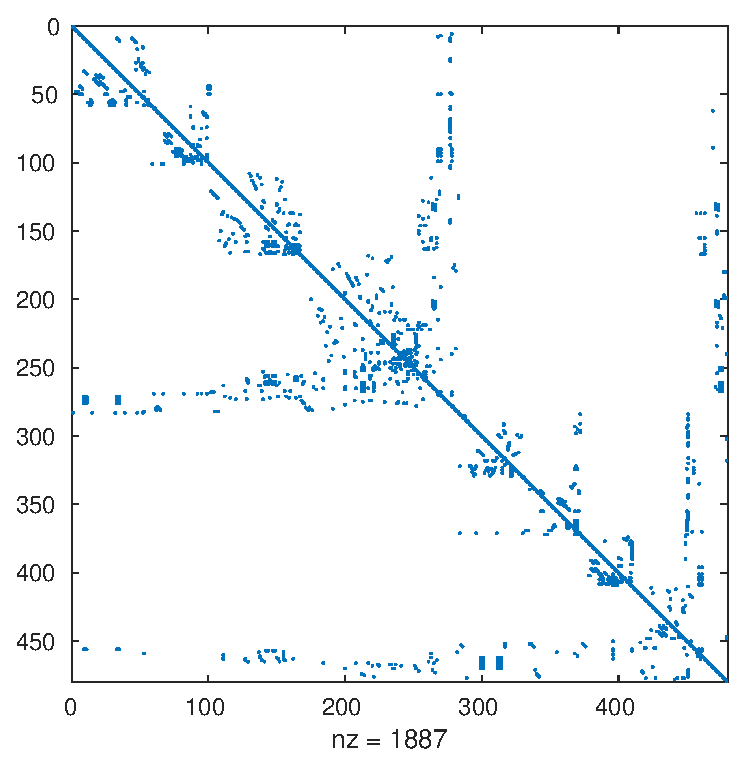
\includegraphics[width=0.95\textwidth]{figures/west0479-match-metis} 
% \end{center}  
%\end{minipage}
%    \caption{Application of multilevel
%nested dissection after the matrix is already rescaled and permuted using maximum weight matching.}
%    \label{fig:metis}
%\end{figure}



%\textbf{Theorem 1 (Residue Theorem).}
%Let $f$ be analytic in the region $G$ except for the isolated singularities $a_1,a_2,\ldots,a_m$. If $\gamma$ is a closed rectifiable curve in $G$ which does not pass through any of the points $a_k$ and if $\gamma\approx 0$ in $G$ then
%\[
%\frac{1}{2\pi i}\int_\gamma f = \sum_{k=1}^m n(\gamma;a_k) \text{Res}(f;a_k).
%\]
%\textbf{Theorem 2 (Maximum Modulus).}
%\emph{Let $G$ be a bounded open set in $\mathbb{C}$ and suppose that $f$ is a continuous function on $G^-$ which is analytic in $G$. Then}
%\[
%\max\{|f(z)|:z\in G^-\}=\max \{|f(z)|:z\in \partial G \}.
%\]